\documentclass[tikz,border=3pt]{standalone}
\usepackage[utf8]{inputenc}
\usepackage[T1]{fontenc}
\usepackage{lmodern}
\renewcommand{\familydefault}{\sfdefault}
\usepackage{sansmath}\sansmath
\usepackage{chemfig}
\usepackage{pgfplots}\pgfplotsset{compat=1.18,/pgf/number format/use comma,/pgf/number format/1000 sep={.}}
\usetikzlibrary{arrows.meta,calc,positioning,decorations.pathmorphing,patterns}
% paleta del sitio
\definecolor{nar}{HTML}{E8680C}\definecolor{narc}{HTML}{FFB35C}\definecolor{hielo}{HTML}{FFF3E8}
\definecolor{tinta}{HTML}{1D1D1F}\definecolor{gris}{HTML}{6E6E73}\definecolor{lila}{HTML}{7C5CF0}
\definecolor{azul}{HTML}{2F6FD6}\definecolor{menta}{HTML}{17A673}\definecolor{coral}{HTML}{E8342A}
\begin{document}
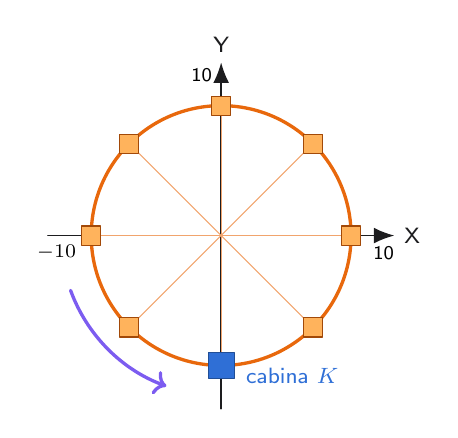
\begin{tikzpicture}[font=\small,x=0.55cm,y=0.55cm,line cap=round,line join=round,step={(1,1)}]
\draw[-{Latex[length=2.6mm,width=2mm]},tinta,semithick] (-4,0)--(4,0) node[right,font=\footnotesize] {X};
\draw[-{Latex[length=2.6mm,width=2mm]},tinta,semithick] (0,-4)--(0,4) node[above,font=\footnotesize] {Y};
\draw[nar,very thick] (0,0) circle (3);
\draw[nar!60] (0,0)--(0:3);
\draw[nar!60] (0,0)--(45:3);
\draw[nar!60] (0,0)--(90:3);
\draw[nar!60] (0,0)--(135:3);
\draw[nar!60] (0,0)--(180:3);
\draw[nar!60] (0,0)--(225:3);
\draw[nar!60] (0,0)--(270:3);
\draw[nar!60] (0,0)--(315:3);
\filldraw[fill=narc,draw=nar!70!black] (0:3) ++(-0.22,-0.22) rectangle ++(0.44,0.44);
\filldraw[fill=narc,draw=nar!70!black] (45:3) ++(-0.22,-0.22) rectangle ++(0.44,0.44);
\filldraw[fill=narc,draw=nar!70!black] (90:3) ++(-0.22,-0.22) rectangle ++(0.44,0.44);
\filldraw[fill=narc,draw=nar!70!black] (135:3) ++(-0.22,-0.22) rectangle ++(0.44,0.44);
\filldraw[fill=narc,draw=nar!70!black] (180:3) ++(-0.22,-0.22) rectangle ++(0.44,0.44);
\filldraw[fill=narc,draw=nar!70!black] (225:3) ++(-0.22,-0.22) rectangle ++(0.44,0.44);
\filldraw[fill=narc,draw=nar!70!black] (315:3) ++(-0.22,-0.22) rectangle ++(0.44,0.44);
\filldraw[fill=azul,draw=azul!70!black] (0,-3) ++(-0.3,-0.3) rectangle ++(0.6,0.6);
\node[right,font=\footnotesize,text=azul] at (0.35,-3.25) {cabina $K$};
\node[font=\scriptsize] at (3.75,-0.4) {10}; \node[font=\scriptsize] at (-0.45,3.7) {10};
\node[font=\scriptsize] at (-3.8,-0.4) {$-10$};
\draw[lila,very thick,->] (200:3.7) arc (200:250:3.7);
\end{tikzpicture}
\end{document}
